\chapter*{Basketball \label{chap:basketball}}

In IUF competition, unicycle basketball is played using the international rules for regular basketball with a few changes.
The items below, in combination with standard international basketball rules, are what are used for Unicon competition.

\section{Unicycles}
The maximum wheel size is 640mm (25.2$"$).
The unicycles must not have sharp or protruding parts anywhere that might
cause injuries.
Quick-release levers and bolts, for example, must be folded back and not excessively long.
The pedals must be plastic or rubber.

\section{Violations}
A violation occurs when the player breaks one of the rules of Basketball.
A violation results in the awarding of the ball to the opposing team.
Examples of violations include traveling, double dribble, backcourt violation, palming the ball, and stepping out of bounds.

\section{Clothing}
Shoes must be worn.
All players of a team must wear shirts of the same color.
The color must be clearly different from the opponent's color.
At tournaments and other large events each team should have two different colored sets of shirts.

Clothing suggestions for comfort and safety:
\begin{itemize}
\item Short shoe laces, or laces tucked in
\item Definitely no jewelry (watches, necklaces, earrings)
\end{itemize}

\section{Fouls}
A foul is an illegal action that can be committed by a player from one team against a player from the opposing team.
If contact occurs beyond what is deemed to be reasonable, or if a player thereby obtains an unfair advantage from it, a foul is committed.
Examples of fouls include pushing, tripping, striking or holding an opposing player and unsportsmanlike conduct.
A foul results in the awarding of the ball to the opposing team and/or free throws.

\section{Steps And Traveling}
A traveling violation occurs when a player holding the ball steps in excess of the prescribed limits.
A step is a half revolution of the wheel; meaning that each wheel revolution is the equivalent of two steps because pedaling with one leg only moves the wheel half a revolution.
After a player establishes a pivot foot (the bottom foot of an idle), the player may not switch the idle foot or take a step unless he begins dribbling.
If a player is in the act of passing or shooting the ball, then the player is allowed to take one full step without dribbling.

\section{Idling, Twisting and Hopping}
Idling is equivalent to the pivot foot and therefore is allowed.
Twisting, where the pedals stay at the same height, while you move the unicycle left and right is also considered your pivot foot, and therefore allowed.
The player must also stay within a one-meter radius from the point where the idling or twisting started.
A player may not hop (jump up and down repeatedly with the unicycle) while holding the ball.
Hopping while dribbling is permitted.

\section{Mounted Player}
The player can only play the ball while mounted on the unicycle.
A player has established position on the unicycle (``mounted'') when the player is sitting on the seat, with both feet on the pedals, and is not touching anything else for support.
Once a player is mounted, the player is considered mounted until some part of his body touches the ground.
The player throwing the ball inbound must be mounted.

\section{Unmounted Player}
If contact is made between the ball and an unmounted player or unicycle, the ball shall be awarded to the other team.
Referees may allow incidental contact between the ball and an unmounted player or unicycle if such contact does not disrupt the flow of the game.
An unmounted player must move himself and his unicycle out of the way as soon as possible
without disrupting the flow of play.
If not possible, the player must leave the unicycle where it lands until it can be retrieved without being disruptive.
A violation will result in an obstruction foul.

An unmounted player's unicycle is considered part of the player.
For the purposes of fouls, a stationary riderless unicycle is considered to have established position; a riderless unicycle that is moving is considered to be out of control.
Thus, if another player is hit by a moving abandoned unicycle, a foul will be called.
If an unmounted player intentionally attempts to play the ball or impede another player, a technical foul will be called.

\section{Four Second Zone}
The three-second zone becomes the four-second zone.

\section{Contact of the Ball with a Unicycle}
It is a violation for a player to intentionally strike or stop the ball with any part of his unicycle or leg, however, incidental contact with a player's unicycle or legs is not a violation.
As long as the player is in contact with the unicycle, riding or not, it is considered part of a player when a ball bounces out of bounds off the unicycle.
If this happens the other team receives possession of the ball.

\section{Ball on Floor}
Any player may pick up a ball that is rolling or stopped on the ground.
This can be dangerous, so care must be taken not to foul a player that is bent over to pick up the ball.
A player may stop a rolling ball with their hand or push a stopped ball to a teammate to pick up.

\newpage

\section{Referee Signals}

\textbf{Administrative signals:}

\begin{figure}[h]
\includegraphics[scale=0.6]{1-a_signal}
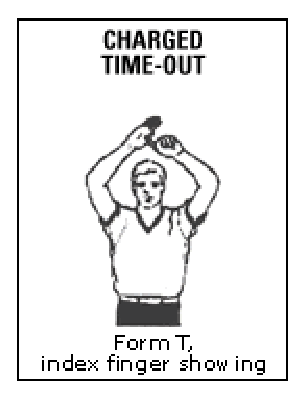
\includegraphics[scale=0.6]{1-b_signal}
\end{figure}

\textbf{Scoring signals:}
\begin{figure}[h]
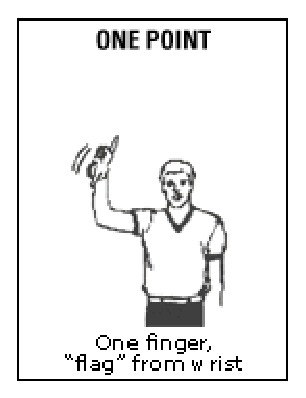
\includegraphics[scale=0.6]{2-a_signal}
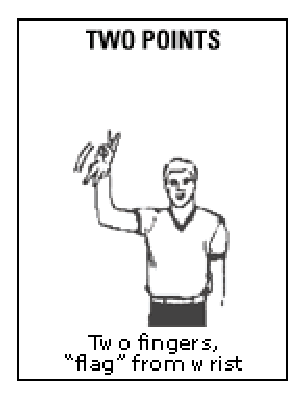
\includegraphics[scale=0.6]{2-b_signal}
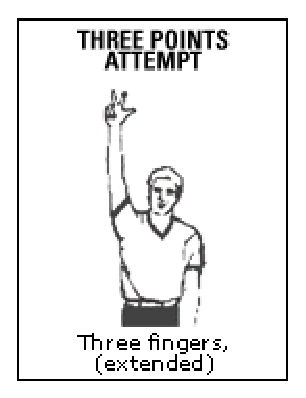
\includegraphics[scale=0.6]{2-c_signal}
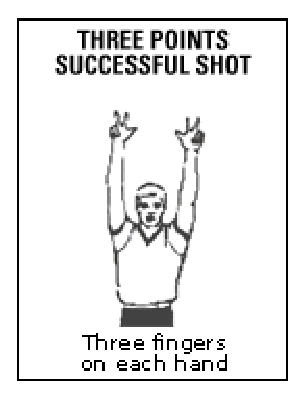
\includegraphics[scale=0.6]{2-d_signal}
\end{figure}

\textbf{Violation signals:}

\begin{figure}[h]
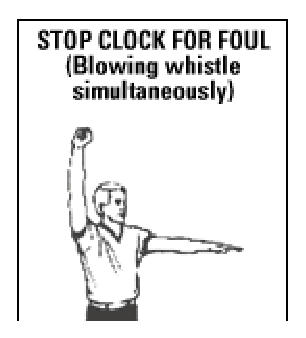
\includegraphics[scale=0.6]{3-a_signal}
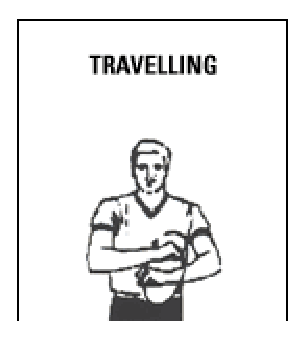
\includegraphics[scale=0.6]{3-b_signal}
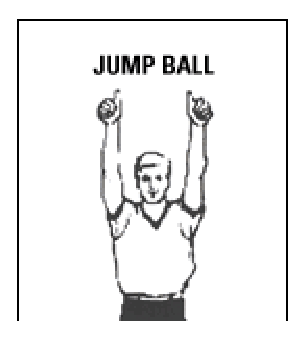
\includegraphics[scale=0.6]{3-c_signal}

\end{figure}
